


\chapter{Appendix - Interaktion mellan student och artificiell intelligens}


I appendix D beskrivs hur förutsägelsen presenterades för studenterna och därefter presenteras formuläret som användes för att undersöka deltagarnas tilltro till förutsägelserna. Till sist redogörs resultatet av formuläret i form av ett stapeldiagram.


\section{Exempel på förutsägelse i interaktion mellan student och artificiell intelligens}
\label{app:AI-test-figur}
Nedan presenteras ett exempel på hur förutsägelsen för en deltagande student såg ut. Exemplet börjar med en övergripande text över hur prognosen har tagits fram och därefter följer förutsägelsen. Studenten får information om vad den artificiella intelligensen tror om att den kommer bli godkänd eller underkänd samt förutsagd tentamenspoäng. Presentationen inkluderar en figur för att visuellt framföra hur förutsägelsen ser ut. 
\begin{figure}[hbtp]
    \centering
    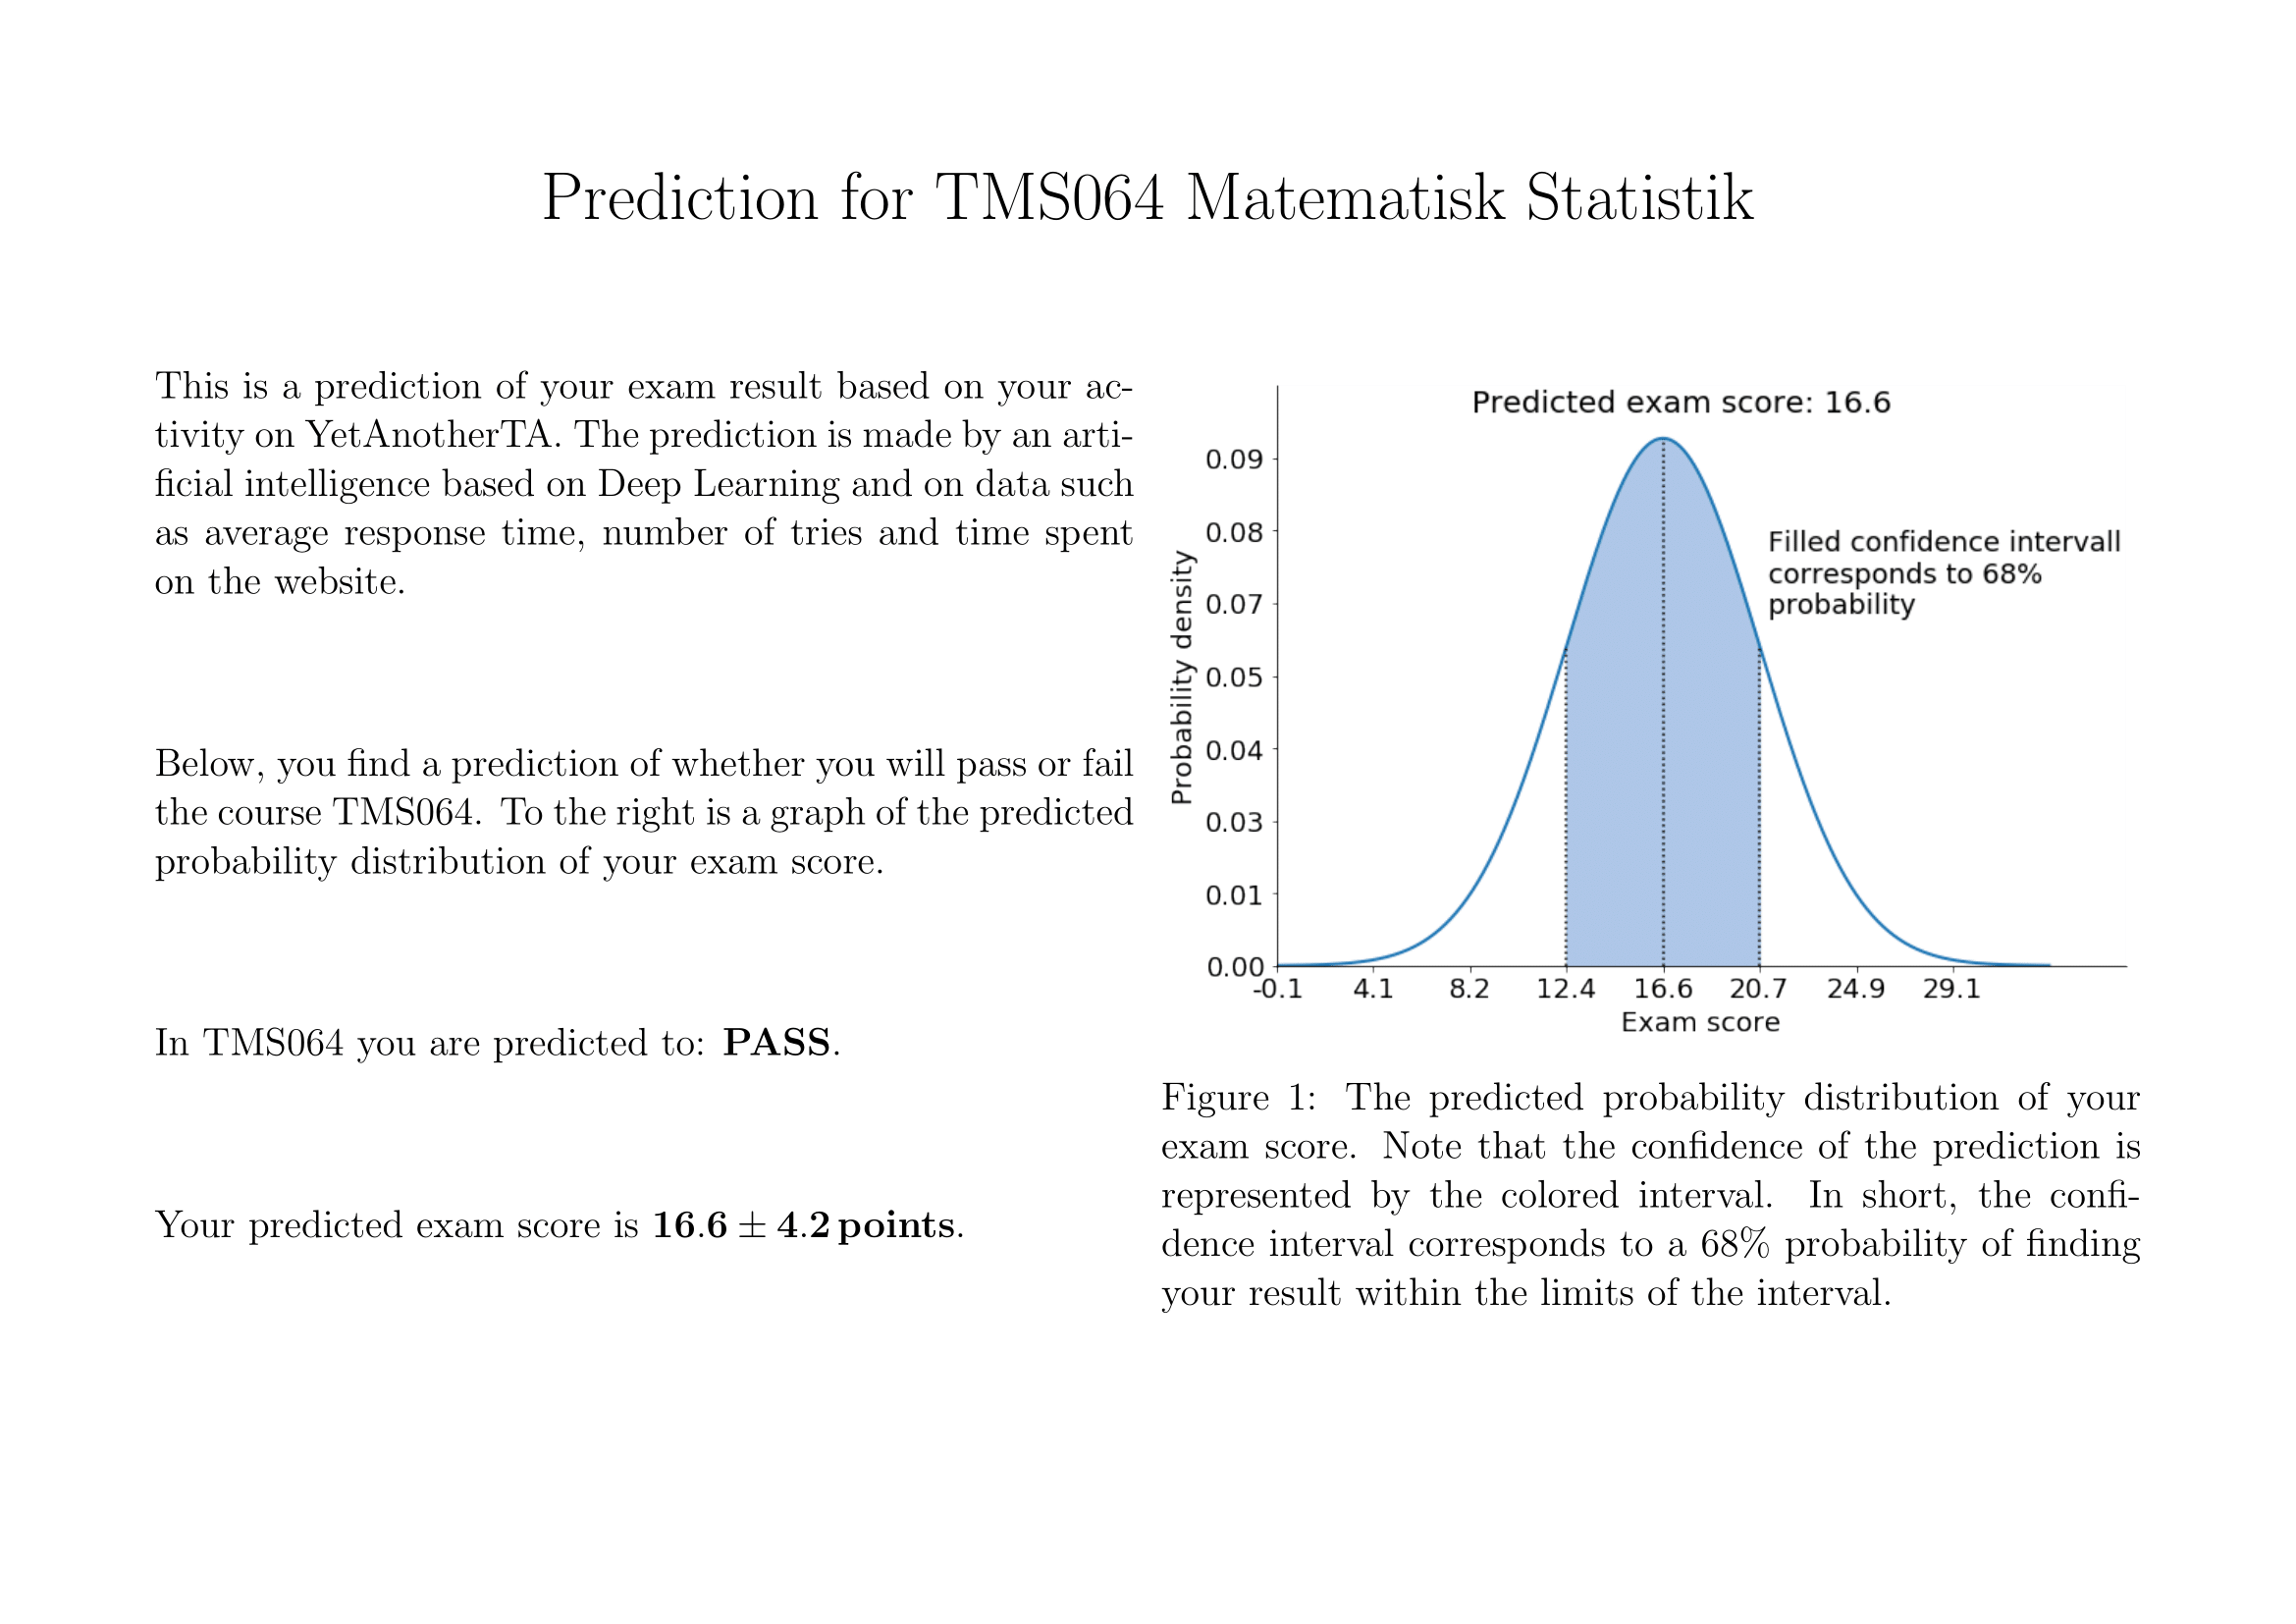
\includegraphics[page=1,scale=0.22]{appendix/AI-test-rapport.png}
    \caption{Exempel på förutsägelse som gavs till en av deltagarna i undersökningen.}
    \label{fig:AI-bild}
\end{figure}

\newpage

\section{Tillitsformulär}
\label{app:AI-test}

För att utvärdera graden av tillit studenterna hade till förutsägelsen användes ett tillitsformulär med 14 påståenden. Varje påstående besvarades med hjälp av en skala från ett till sju, där ett indikerade att man inte höll med påståendet medan sju antydde att man fullständigt höll med.


%\begin{figure}[hbtp]
%    \centering
%    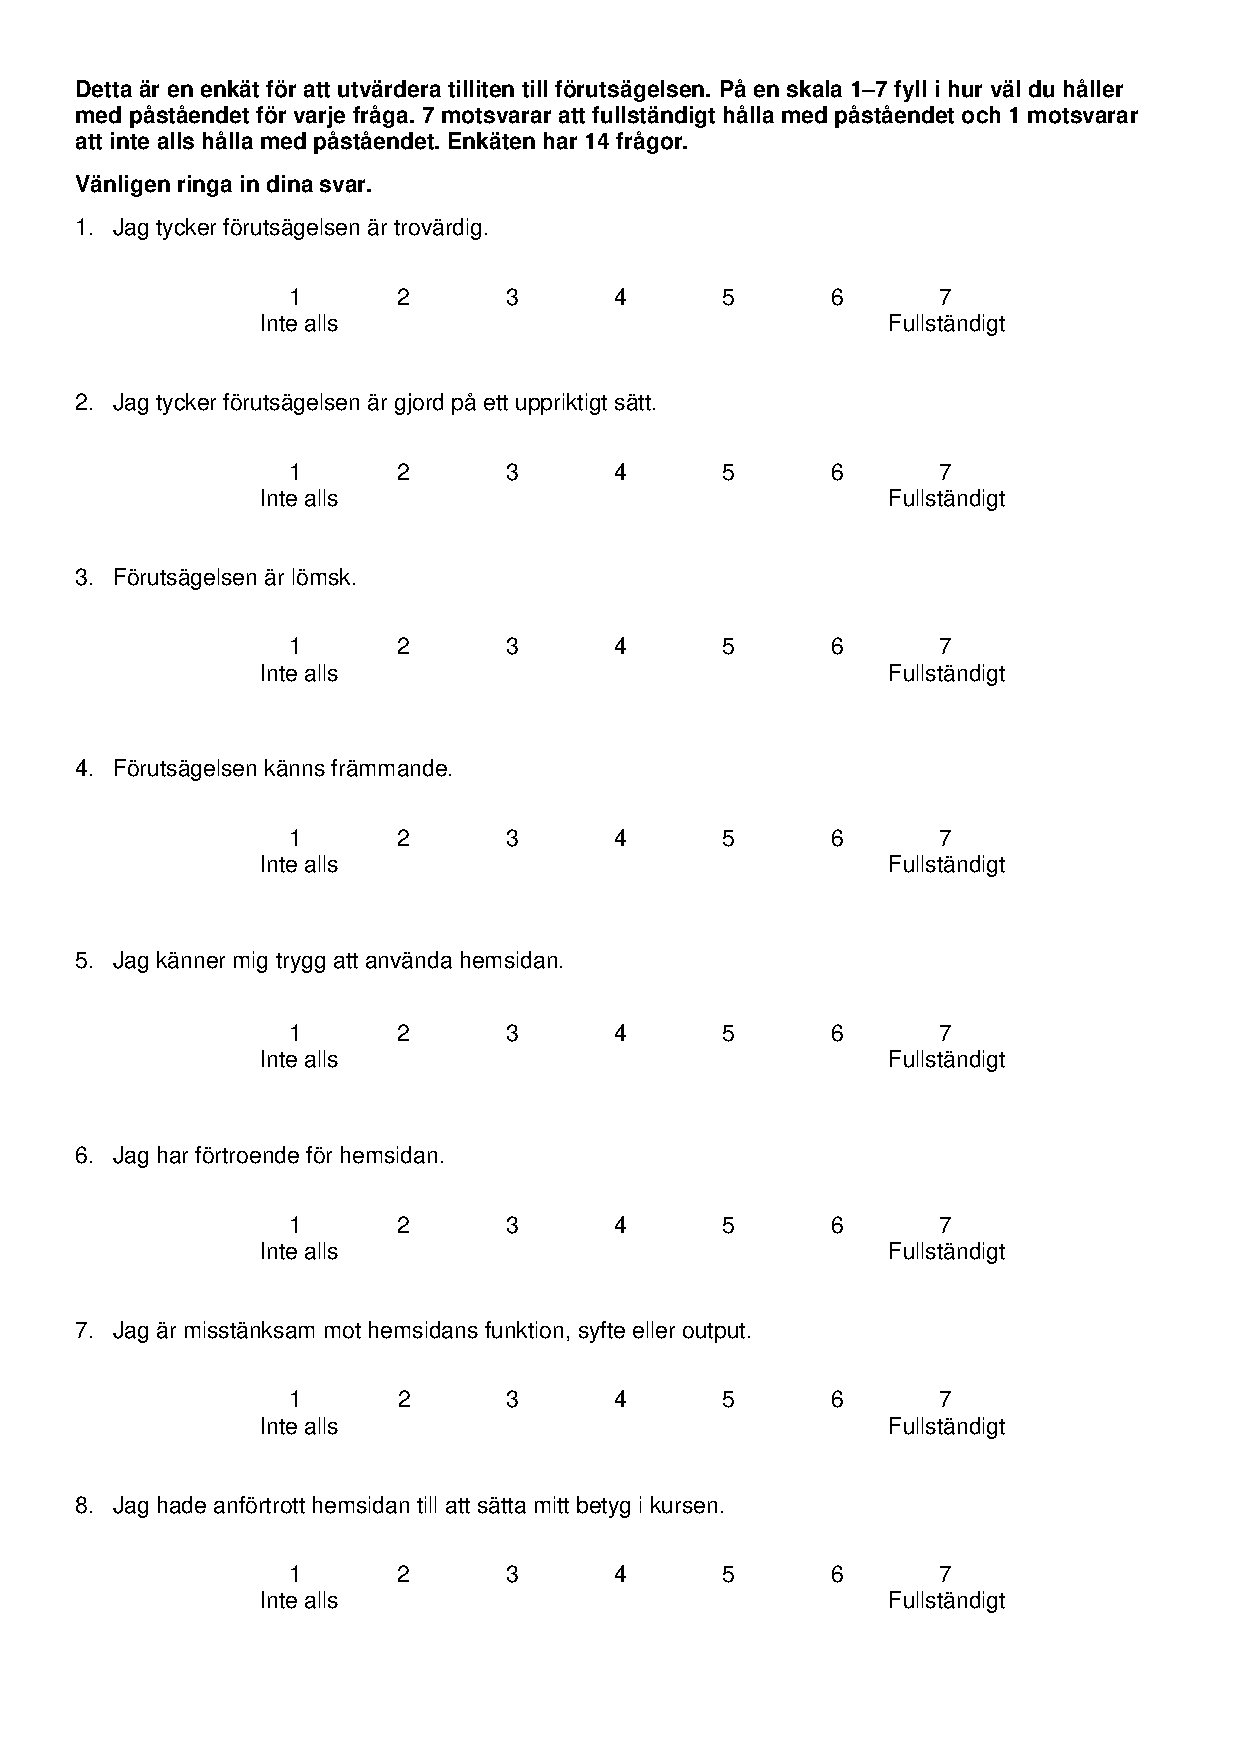
\includegraphics[page=1,scale=0.65]{appendix/tillit_form.pdf}
%   \caption*{Tillitsformulär sida 1.}
%   \label{fig:form1}
%\end{figure}

%\begin{figure}
%    \centering
%    \includegraphics[page=2,scale=0.65]{appendix/tillit_form.pdf}
%    \caption*{Tillitsformulär sida 2}
%    \label{fig:form2}
%\end{figure}



\begin{figure}[htp]
    \centering
    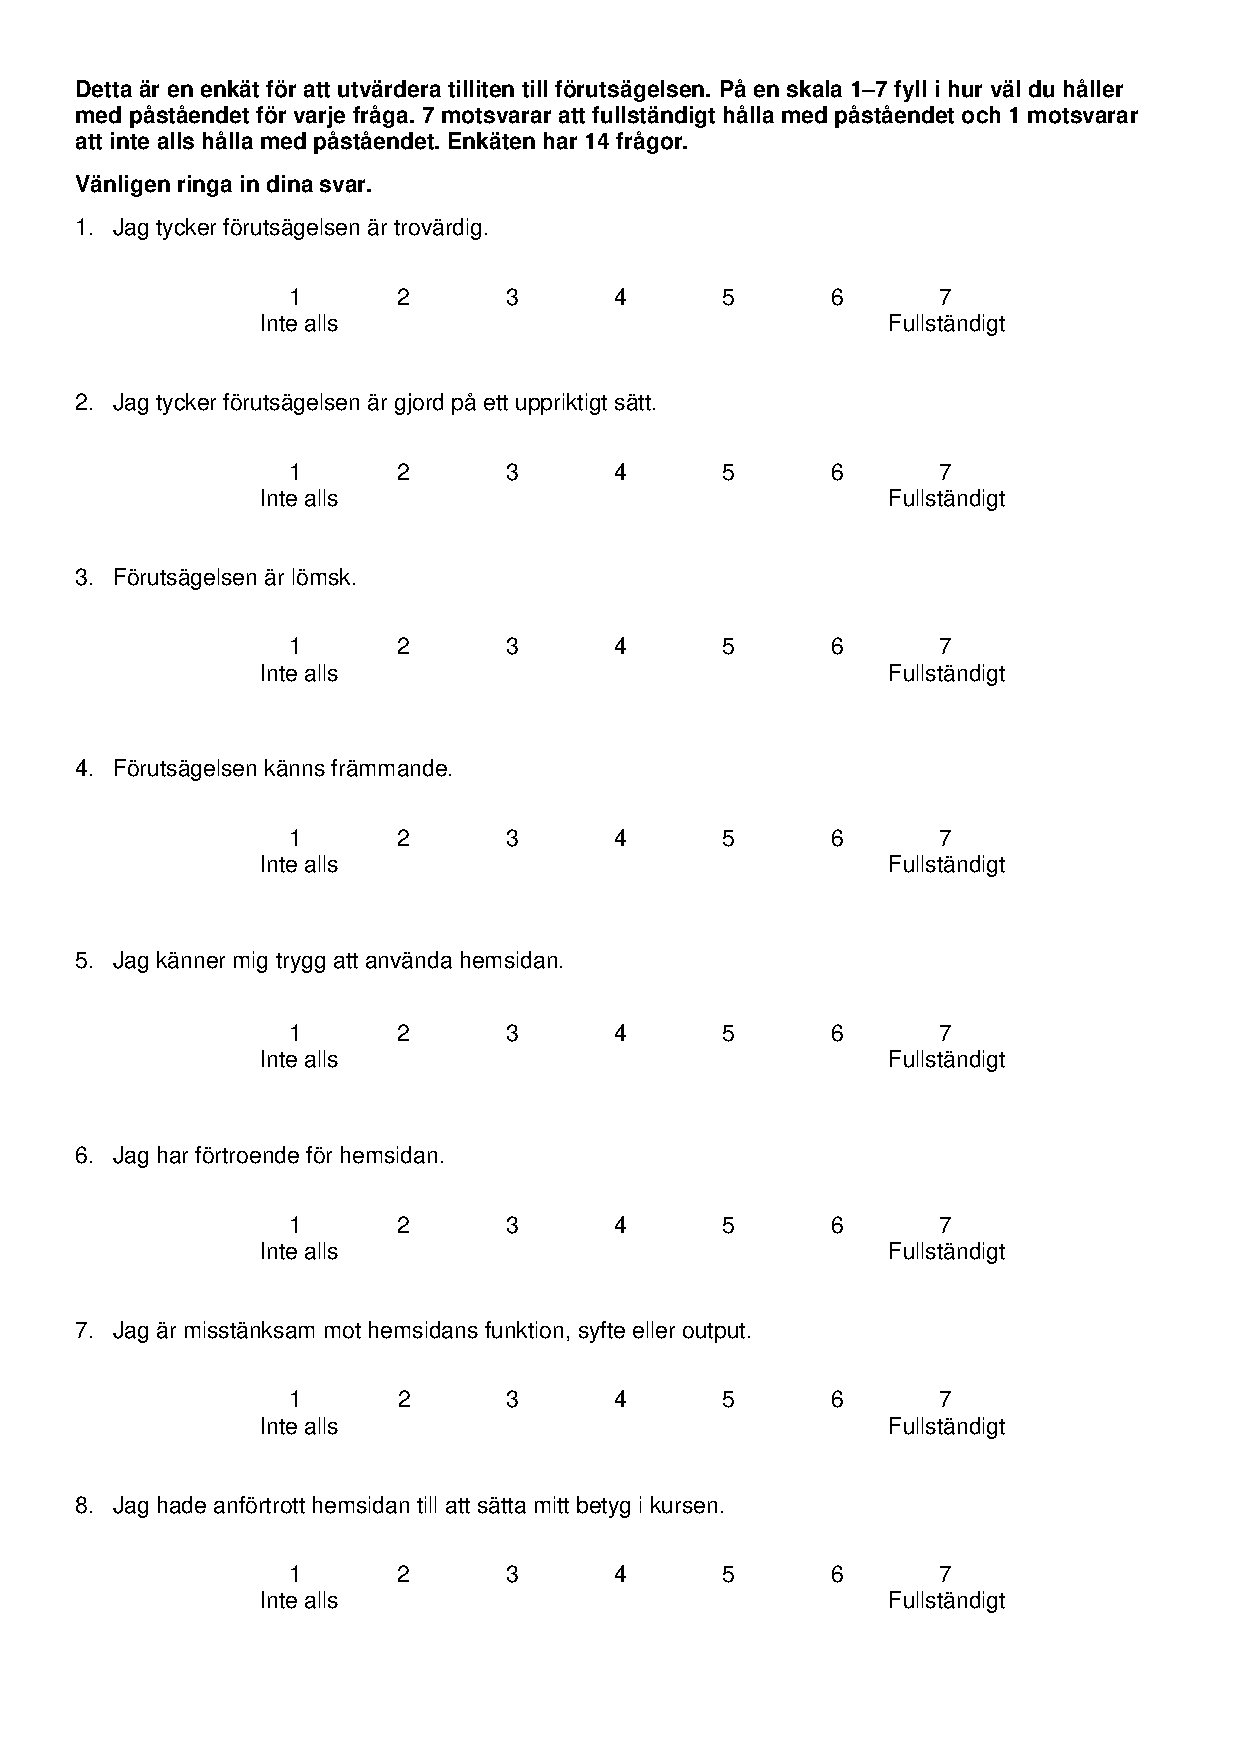
\includegraphics[page=1,scale=0.8]{appendix/tillit_form.pdf}
    \caption*{Tillitsformulär, Sida 1}
    \label{fig:tillit_form1}
\end{figure}

\begin{figure}[htp]
    \centering
    \includegraphics[page=2,scale=0.8]{appendix/tillit_form.pdf}
    \caption*{Tillitsformulär, Sida 2}
    \label{fig:tillit_form2}
\end{figure}

% Alternativ för att få dem på samma sida. 

%\begin{figure}%
%    \centering
%    \subfloat{{Sida 2}{\includegraphics[page=2,scale=0.6,angle=90]{appendix/tillit_form.pdf}}}%
%    \qquad
%    \subfloat{{Sida 1}{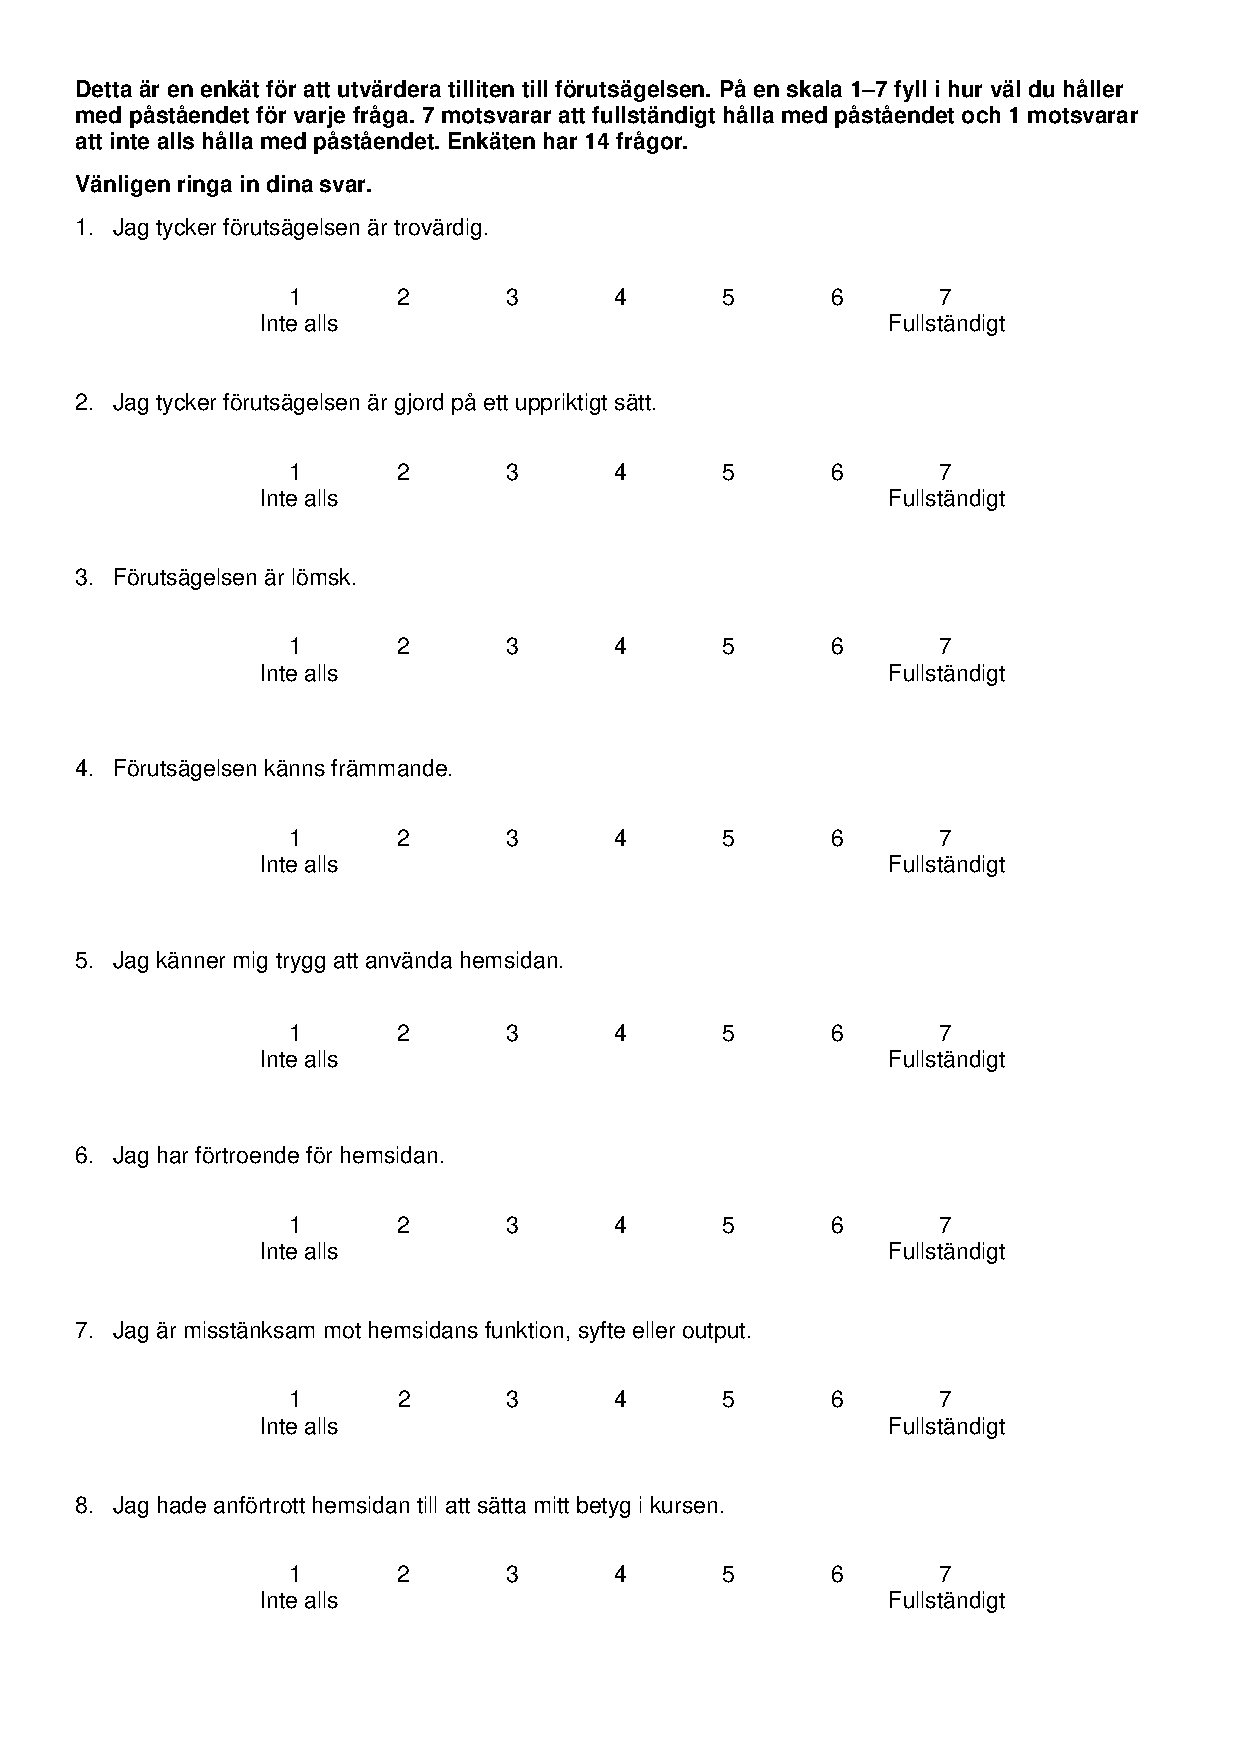
\includegraphics[page=1,scale=0.6,angle=90]{appendix/tillit_form.pdf} }}%
%    %\caption{2 Figures side by side}%
%    \label{fig:openform2-3}%
%\end{figure}

\section{Resutlat av tillitsformuläret}
\label{app:resultattillit}
I figur nedan presenteras svaren på tillitsformuläret från fyra studenter i ett stapeldiagram. Vi noterar att studenterna har stort förtroende för hemsidan, den känns trovärdig och de förstår syftet med förutsägelsen. De tycker däremot inte att den speglar deras betyg i kursen och att förutsägelsen inte är trovärdig. För att dra mer noggranna slutsatser krävs svar från en större mängd studenter.


\begin{figure}[hbtp]
    \centering
    \resizebox {\textwidth} {!} {
        \definecolor{klight_green}{RGB}{196,225,144}
\definecolor{kgreen}{RGB}{94,173,97}
\definecolor{kdark_green}{RGB}{29,122,33}
\definecolor{kgrey}{RGB}{222,222,222}
\definecolor{ktest_green}{RGB}{234,245,179}
\definecolor{kpurple}{RGB}{113,94,181}

% \pgfplotstableread[row sep=\\,col sep=&]{
%     interval & u & false \\
%     U     & 69  & 31 \\
%     3     & 83 & 17  \\
%     4     &    &     \\
%     5     &    &     \\
%     }\mydata

\begin{tikzpicture}
    \begin{axis}[
            ybar,
            x=2cm,
            enlarge x limits={abs=1cm},
            %enlarge y limits={abs=0.5cm},
            bar width=0.2cm,
            width=32cm,
            height=10cm,
            legend style={at={(0.5, 1.2)},
                anchor=north,legend columns=-1},
            legend image post style={scale=2},
            symbolic x coords={1, 2, 3,4,5,6,7,8,9,10,11,12,13,14},
            xtick=data,
            major x tick style = transparent,
            ymajorgrids = true,
            %nodes near coords={\pgfmathprintnumber[fixed,precision=0]{\pgfplotspointmeta}\,\%},
            nodes near coords align={vertical},
            ymin=0,ymax=7.5,
            yticklabel={\pgfmathparse{\tick}\pgfmathprintnumber{\pgfmathresult}},
            ylabel={\small Skattning},
            xlabel={\small Fråga},
            %ticklabel style = {font=\tiny},
            nodes={scale=2, transform shape}  % increase size of everything
        ]
        \addplot [fill=ktest_green!100,draw=kgrey!100] coordinates {(1,3) (2,2) (3,3) (4,2) (5,5) (6,5) (7,1) (8,1) (9,3) (10,1) (11,2) (12,4) (13,4) (14,4)};  % Anv. 1
        \addplot [fill=klight_green!100,draw=kgrey!100] coordinates {(1,1) (2,6) (3,4) (4,3) (5,7) (6,6) (7,1) (8,1) (9,2) (10,1) (11,1) (12,7) (13,1) (14,2)};  % Anv. 2
        \addplot [fill=kgreen!100,draw=kgrey!100] coordinates {(1,5) (2,7) (3,1) (4,1) (5,7) (6,5) (7,1) (8,4) (9,1) (10,1) (11,2) (12,6) (13,5) (14,5)};   % Anv. 3
        \addplot [fill=kdark_green!100,draw=kgrey!100] coordinates {(1,1) (2,7) (3,1) (4,1) (5,7) (6,4) (7,1) (8,3) (9,1) (10,1) (11,4) (12,5) (13,1) (14,3)};   % Anv. 4
        \addplot [fill=kpurple!100,draw=kgrey!100] coordinates {(1,2.5) (2,5.5) (3,2.25) (4,1.75) (5,6.5) (6,5) (7,1) (8,2.25) (9,1.75) (10,1) (11,2.25) (12,5.5) (13,2.75) (14,3.5)};   % Medel
        \legend{Stud. 1, Stud. 2, Stud. 3, Stud. 4, Medel}
    \end{axis}
\end{tikzpicture}
    }
    \caption{Stapeldiagram för enkätsvaren på påstående 1 till 14. Staplarnas höjd representerar deltagarnas skattningar på påståendenas riktighet utefter en sjugradig skalan. De fyra staplarna till vänster för varje påstående representerar deltagarnas svar och den femte till höger anger svarens medelvärde.}
    \label{fig:form_answers}
\end{figure}